\documentclass[border=10pt]{standalone}
\usepackage[svgnames]{xcolor}
\usepackage{amsmath}
\usepackage{pgfplots}
\pgfplotsset{compat=newest}
\usepackage[sfdefault]{FiraSans}
\usepackage{FiraMono}
\renewcommand*\familydefault{\sfdefault}
\begin{document}
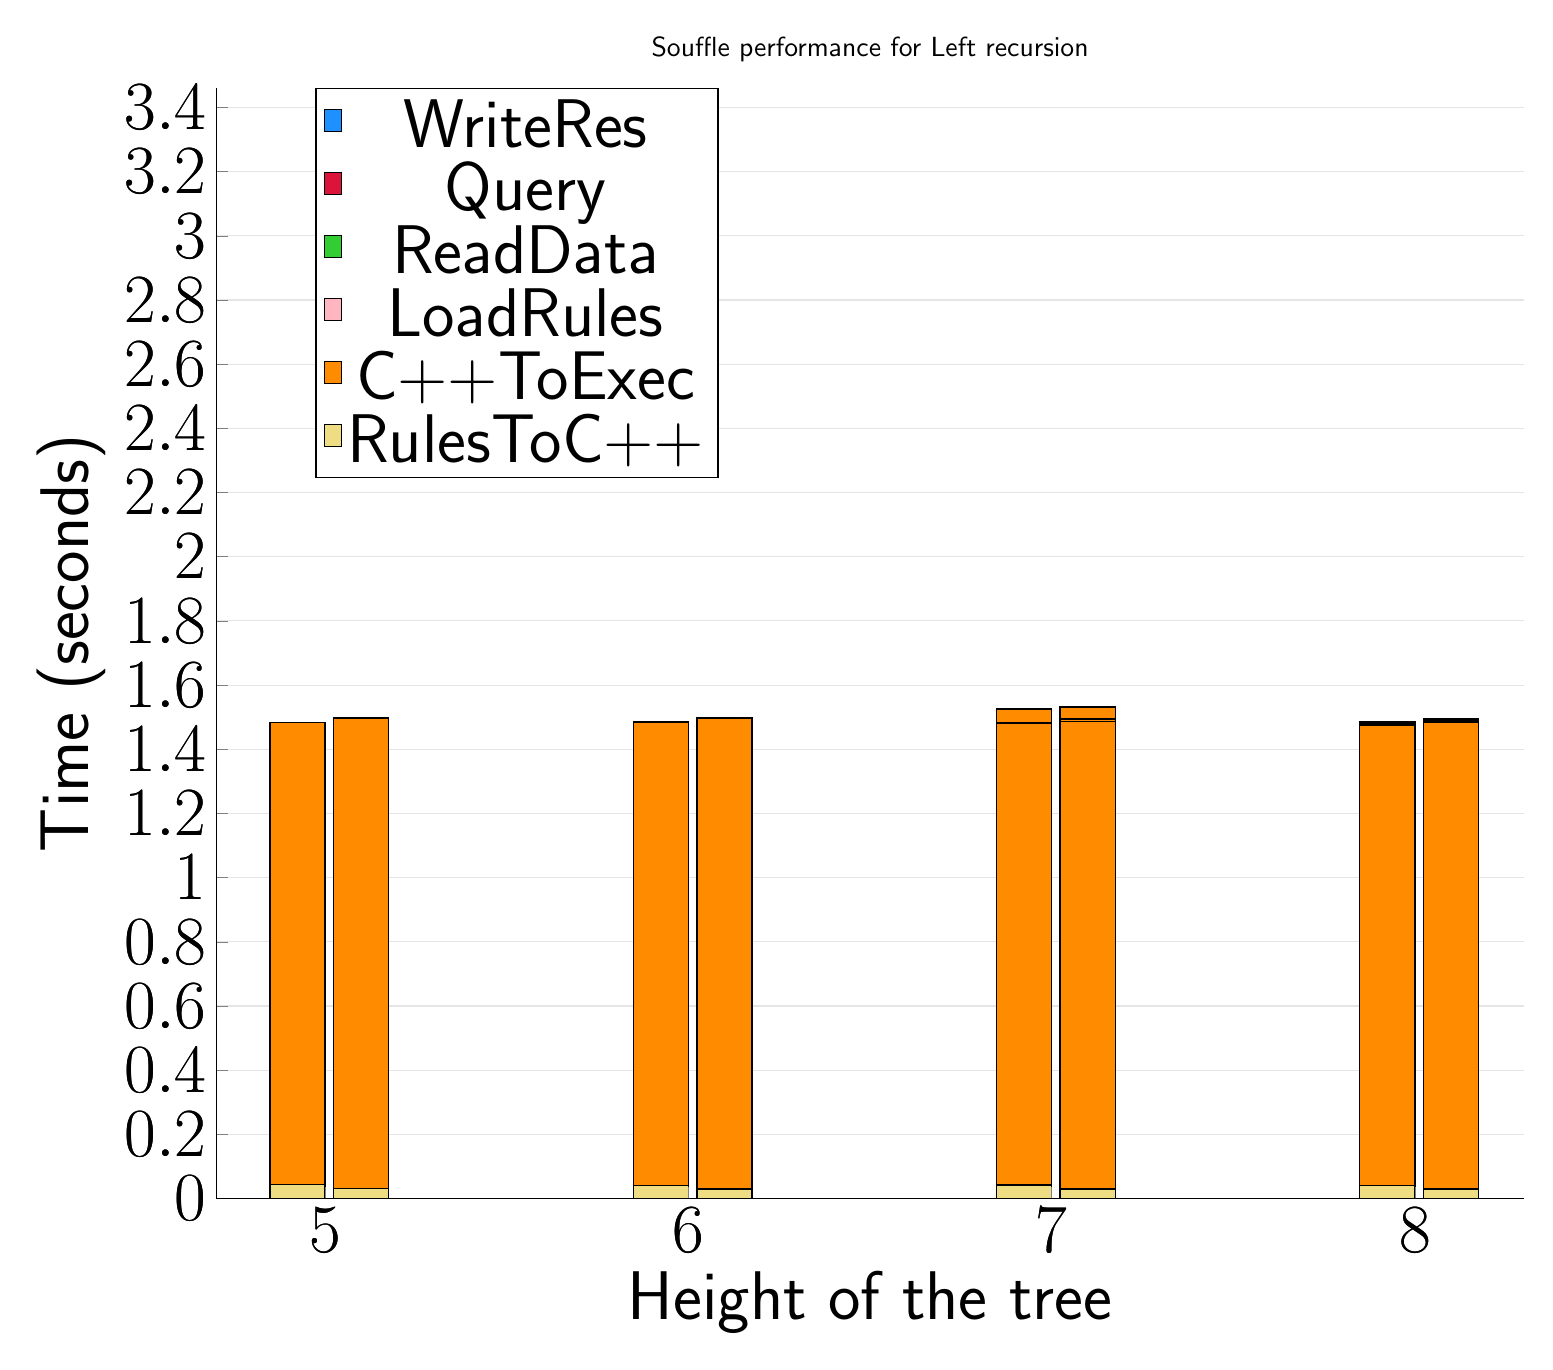
\begin{tikzpicture}
	\begin{axis}[
			ybar stacked,
			title={Souffle performance for Left recursion},
			bar shift=-10pt,
			width=1.5\textwidth,
			bar width=0.7cm,
			ymajorgrids, tick align=inside,
			major grid style={draw=gray!20},
			xtick=data,
			ymin=0, ymax=3.4609999895095824,
			axis x line*=bottom,
			axis y line*=left,
			enlarge x limits=0.1,
			legend style={
					at={(0.23, 1)},
					anchor=north,
					legend columns=1,
					font=\Huge,
				},
			ylabel={Time (seconds)},
			xlabel={Height of the tree},
			label style={font=\Huge},
			tick label style={font=\Huge},
		]
		\addlegendimage{fill=DodgerBlue, draw=black, line width=0.2pt}
		\addlegendentry{WriteRes}
		\addlegendimage{fill=Crimson, draw=black, line width=0.2pt}
		\addlegendentry{Query}
		\addlegendimage{fill=LimeGreen, draw=black, line width=0.2pt}
		\addlegendentry{ReadData}
		\addlegendimage{fill=LightPink, draw=black, line width=0.2pt}
		\addlegendentry{LoadRules}
		\addlegendimage{fill=DarkOrange, draw=black, line width=0.2pt}
		\addlegendentry{C++ToExec}
		\addlegendimage{fill=LightGoldenrod, draw=black, line width=0.2pt}
		\addlegendentry{RulesToC++}
		\addplot +[fill=LightGoldenrod, draw=black, line width=0.5pt] coordinates {
				(5, 0.042999982833862305)
				(6, 0.039999985694885255)
				(7, 0.04200005531311035)
				(7, 0.04000000953674317)
				(7, 0.04000000953674317)
				(8, 0.039999961853027344)
				(8, 0.039999961853027344)
				(8, 0.04000000953674317)
			};
		\addplot +[fill=DarkOrange, draw=black, line width=0.5pt] coordinates {
				(5, 1.4400000095367431)
				(6, 1.4450000047683715)
				(7, 1.4839999675750732)
				(7, 1.4420000314712524)
				(7, 1.4399999856948853)
				(8, 1.4360000371932984)
				(8, 1.4430000543594361)
				(8, 1.4390000104904175)
			};
		\addplot +[fill=LightPink, draw=black, line width=0.5pt] coordinates {
				(5, 0.00012110810000000001)
				(6, 0.0001315124)
				(7, 9.33836e-05)
				(7, 9.51542e-05)
				(7, 0.0001210961)
				(8, 9.81916e-05)
				(8, 9.94125e-05)
				(8, 0.0001242207)
			};
		\addplot +[fill=LimeGreen, draw=black, line width=0.5pt] coordinates {
				(5, 0.00030939179999999995)
				(6, 0.00043649180000000006)
				(7, 0.0004757792)
				(7, 0.000469996)
				(7, 0.0005174)
				(8, 0.0007679169000000001)
				(8, 0.0007898418)
				(8, 0.0008020498999999999)
			};
		\addplot +[fill=Crimson, draw=black, line width=0.5pt] coordinates {
				(5, 0.0001316583)
				(6, 0.0003765666)
				(7, 0.0007095499)
				(7, 0.0006943293000000001)
				(7, 0.0007842039999999999)
				(8, 0.0018131109999999998)
				(8, 0.001866992)
				(8, 0.0019298580000000002)
			};
		\addplot +[fill=DodgerBlue, draw=black, line width=0.5pt] coordinates {
				(5, 0.00033970049999999997)
				(6, 0.0004907544)
				(7, 0.0005899623000000001)
				(7, 0.0004598209)
				(7, 0.0005094081)
				(8, 0.0009038497999999999)
				(8, 0.0010758501000000002)
				(8, 0.0010101547)
			};
	\end{axis}
	\begin{axis}[
			ybar stacked,
			bar shift=13pt,
			width=1.5\textwidth,
			bar width=0.7cm,
			ymajorgrids, tick align=inside,
			major grid style={draw=none},
			xtick=data,
			ymin=0, ymax=3.4609999895095824,
			axis x line*=none,
			axis y line*=none,
			enlarge x limits=0.1,
			label style={font=\Huge},
			tick label style={font=\Huge},
		]
		\addplot +[fill=LightGoldenrod, draw=black, line width=0.5pt] coordinates {
				(5, 0.031000000000000007)
				(6, 0.030000000000000006)
				(7, 0.030000000000000006)
				(7, 0.031000000000000007)
				(7, 0.030000000000000006)
				(8, 0.030000000000000006)
				(8, 0.030000000000000006)
				(8, 0.030000000000000006)
			};
		\addplot +[fill=DarkOrange, draw=black, line width=0.5pt] coordinates {
				(5, 1.466)
				(6, 1.467)
				(7, 1.501)
				(7, 1.4629999999999999)
				(7, 1.4569999999999996)
				(8, 1.4549999999999998)
				(8, 1.4600000000000002)
				(8, 1.4599999999999997)
			};
		\addplot +[fill=LightPink, draw=black, line width=0.5pt] coordinates {
				(5, 0.00012030000000000001)
				(6, 0.00013050000000000003)
				(7, 8.26e-05)
				(7, 9.44e-05)
				(7, 0.00012029999999999998)
				(8, 9.72e-05)
				(8, 9.859999999999998e-05)
				(8, 0.0001232)
			};
		\addplot +[fill=LimeGreen, draw=black, line width=0.5pt] coordinates {
				(5, 0.0003086)
				(6, 0.00043560000000000007)
				(7, 0.00047410000000000003)
				(7, 0.00046879999999999996)
				(7, 0.0005165)
				(8, 0.0007673999999999999)
				(8, 0.000788)
				(8, 0.0008012999999999999)
			};
		\addplot +[fill=Crimson, draw=black, line width=0.5pt] coordinates {
				(5, 0.00013099999999999999)
				(6, 0.00037610000000000003)
				(7, 0.0007089999999999999)
				(7, 0.0006937)
				(7, 0.0007836)
				(8, 0.0018126999999999998)
				(8, 0.0018664)
				(8, 0.0019291)
			};
		\addplot +[fill=DodgerBlue, draw=black, line width=0.5pt] coordinates {
				(5, 0.0002651)
				(6, 0.00039779999999999997)
				(7, 0.0004694)
				(7, 0.0004426)
				(7, 0.0005087)
				(8, 0.0009031000000000001)
				(8, 0.0009285)
				(8, 0.000932)
			};
	\end{axis}
\end{tikzpicture}

\end{document}
